\chapter{Introduction}
\label{chap:1}
\ChapterPageStuff{1}

\section{Background}\label{section:background}

Software maintenance according to the \textit{IEEE Standard 1219}\footnote{\textbf{IEEE Standards} documents are developed within the Technical Committees of the IEEE Societies and the Standards Coordinating Committees of the IEEE Standards Board \cite{Mamone1994}.} is the process that includes the following phases \cite{Mamone1994, Hasan2012}:
\begin{itemize}
	\item Identifying the problem or modification and classification of it
	\item Analysis of the identification
	\item Design of the solution
	\item Implementation of the solution
	\item System testing of the modified software system
	\item Acceptance test on the fully integrated system
	\item Delivery requirements met of the modified software system
\end{itemize}

Maintenance of software systems is continuous and is a reduced form of software development and is aimed to modify software systems while preserving its integrity \cite{Sneed2004, Ackermann2009}. Software maintenance needs to be done regularly in its entire lifespan. 

\subsection{Maintenance in software systems}
Most companies will strife to increase their digital products and services over the life cycle of the software project and this will increase the maintenance that needs to be done on both new and old systems \cite{Niu2018, Galster2019, Hasan2012}. Although maintenance is important for software systems, most companies don't have a defined maintenance model or process to guide them when implementing maintenance \cite{Stojanov2017}. \par Software maintenance is an essential task in software development, it can directly reduce cost and effort to create new software systems \cite{FrancisThamburaj2017}. According to a study of the total development cost for typical software maintenance efforts, conducted by the United States Department of Commerce found that the cost can be as much as $60\%$-$80\%$ of the total cost of the software systems entire development life cycle of 10 years \cite{Ogheneovo2014, Stark1996, Ackermann2009,Tang2010}. These costs will increase (as in \Cref{fig:CH1_Costs_of_fixing_bugs}) to maintain much older and more complex software systems, therefore it is key to the feasibility of the software systems to implement maintenance on it \cite{Alenezi2016, Booch1986}.

\begin{figure}[h!] % An h :here, t: top, b: bottom.
	\centering % cent the figure
	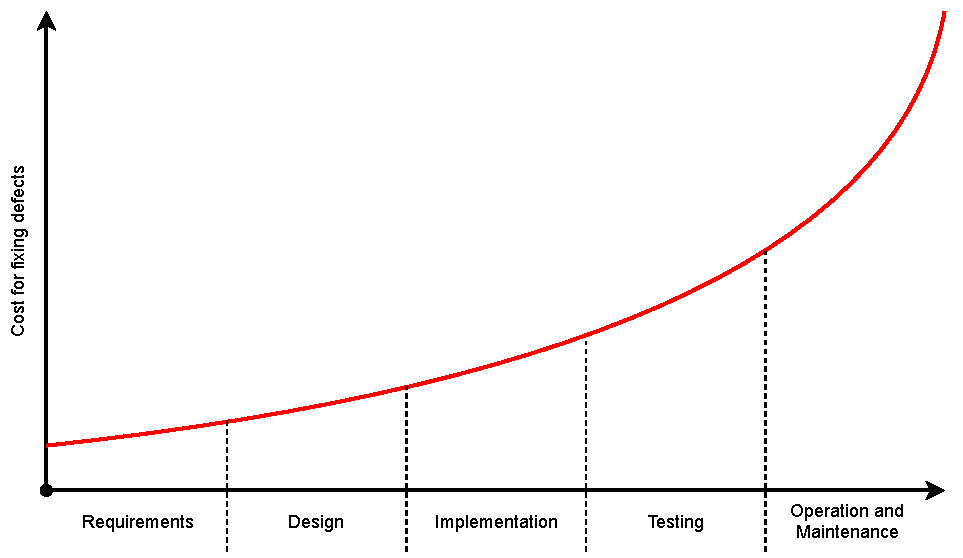
\includegraphics[width=0.5\textwidth]{Images/Chapter1/Background/Cost_of_fixing_bugs/Cost_of_fixing_bugs.pdf}
	\caption[Cost of fixing software system defects]
	{\textit{Cost of fixing software system defects \cite{Ogheneovo2014}}}\label{fig:CH1_Costs_of_fixing_bugs}
\end{figure} 

In \Cref{tbl:CH1_MaintenanceTypes} the adaptive and perfective maintenance types are most effective when maintaining the software integrity of a system. Software maintenance is needed but it can be difficult to prioritise the resources to certain parts of the software system to do maintenance on \cite{Mamone1994, Hasan2012}.

\begin{table}[!htb]
	\centering
	\small
	\caption[Software maintenance types]
	{\textit{Software maintenance types}}
	\label{tbl:CH1_MaintenanceTypes}
	\begin{tabularx}{\textwidth}{|c|X|c|}
		\hline
		\textbf{Maintenance type} & \textbf{Description} & \textbf{$\%$ of maintenance activities} \\ \hline
		Adaptive & \raggedright Adaptive maintenance are any software systems. This also include enhancements to the software systems. & $\approx 35.5\%$ \\ \hline
		Perfective & Perfective maintenance based are modifications made based on the change of the user's requirements. & $\approx 35.5\%$ \\ \hline
		Corrective & \raggedright Corrective maintenance are improvements made to fix certain defects or errors in a software system. & $\approx 20\%$ \\ \hline
		Preventive & \raggedright  Preventive maintenance are improvements made to software systems that prevents problems in the future. & $\approx 5\%$ \\ \hline
	\end{tabularx}
\end{table}

\subsection{Problems with implementing software maintenance}
Under most circumstances maintenance is implemented if a software system does not meet the required functions specified by the performance requirements \cite{Ogheneovo2014, Sneed2004}. These systems will also most likely have multiple software defects or will be extremely complex due to:

\begin{itemize}
	\item \textbf{Problem domain being complex:} The software may not be well defined or structured. This is due how large the software systems grow over its entire life cycle or duplicate software components that are made. This is caused by poor understanding of the system architecture by developers not doing the required maintenance on these systems and just adding new features \cite{Galster2019, Booch1986}.
	\item \textbf{Difficulties of managing development process:} Most companies will strife to increase their digital products and services over the life cycle of the software project to maximise possible profits with the resources invested \cite{Niu2018}. Increasing production of the development process will only strain the efforts of maintaining software systems \cite{Sneed2004}.\par The development team needs to prioritise concrete tasks in the development process to make the project feasible, by just focusing on these tasks poor decisions are made about the required task to perform software maintenance \cite{Galster2019, Ogheneovo2014, Lenarduzzi2017}. 
	\item \textbf{Flexibility of the software:} Trying to predict what the possible future architecture may look like and modifying it while preserving the software's integrity, may be difficult in software maintenance \cite{Garlan1999}. Software is flexible if it is adaptable to the problem domain when adding modifications to it \cite{Ogheneovo2014}.\par Most development teams will follow a software development methodology to create a future architecture that is modular and structured to preserve the development integrity of new software \cite{Vijayasarathy2016, Rehman2018}. This will also have an impact the type of maintenance activity (as in \Cref{tbl:CH1_MaintenanceTypes}) the development team will use which are the called corrective, perfective, adaptive and preventive maintenance \cite{FrancisThamburaj2017, Hasan2012, Stojanov2017, Snipes2018}.
	\item \textbf{Change in the user's requirements:} In software development the users will often request new additional requirements to the software systems that are delivered to them \cite{Ogheneovo2014}. Modifying software systems may include new additional features that change the initial system architecture. Maintenance on these systems are crucial to ensure that existing components of the system will work as intended with the new components that are added.
\end{itemize}

\subsection{Software maintenance model}
A software maintenance model is an abstract representation of the evolution of software systems to keep track of all the maintenance activities when implementing software maintenance \cite{Ren2011}. The \textit{IEEE Standard 1219} for software maintenance is the standard that should be followed when planning the software maintenance as in \Cref{fig:CH1_IEEE_Model}.\par It is important to identify the maintenance that should be done before making which will start with user or developer's request to modify software. A feasibility analysis of any changes that is required is made. Certain amount of resources will be needed to implement maintenance and this will impact the design and implementation phase. System and acceptance testing is important to ensure that the system is still fully functional. After the system is fully tested and approved, it will be available to the user and the maintenance process will start again when there are new improvements made for the software system.

\begin{figure}[!htb] % An h :here, t: top, b: bottom.
	\centering % cent the figure
	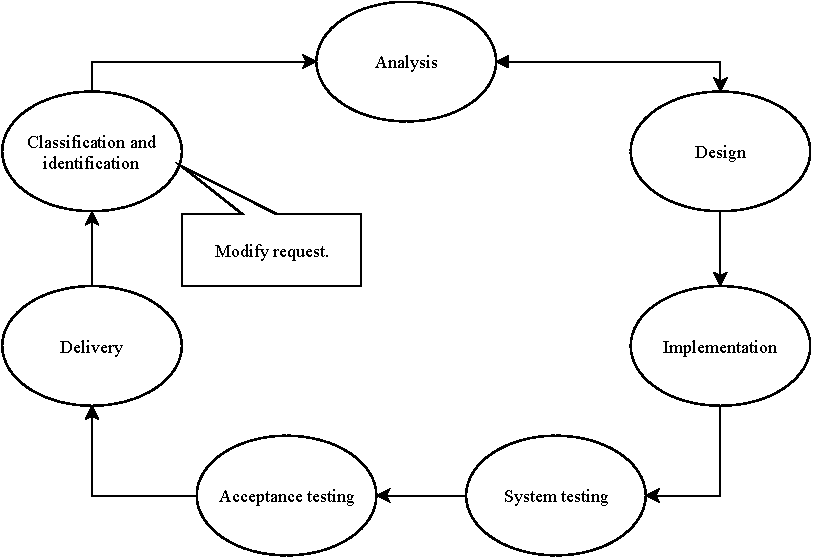
\includegraphics[width=0.6\textwidth]{Images/Chapter1/Background/IEEE_Model/IEEE_Model.pdf}
	\caption[IEEE model]
	{\textit{IEEE model \cite{Ren2011}}} \label{fig:CH1_IEEE_Model}
\end{figure}

To fully follow the \textit{IEEE Standard 1219} of implementing maintenance on a software system, the defects or areas of improvements needs to be identified. Utilisation analysis of event logs can be used to detect any hidden defects or performance issues in a software system to implement software maintenance \cite{Cinque2013, Rong2018a, Levin2019}.

\clearpage


\begin{figure}[!htb] % An h :here, t: top, b: bottom.
	\centering % cent the figure
	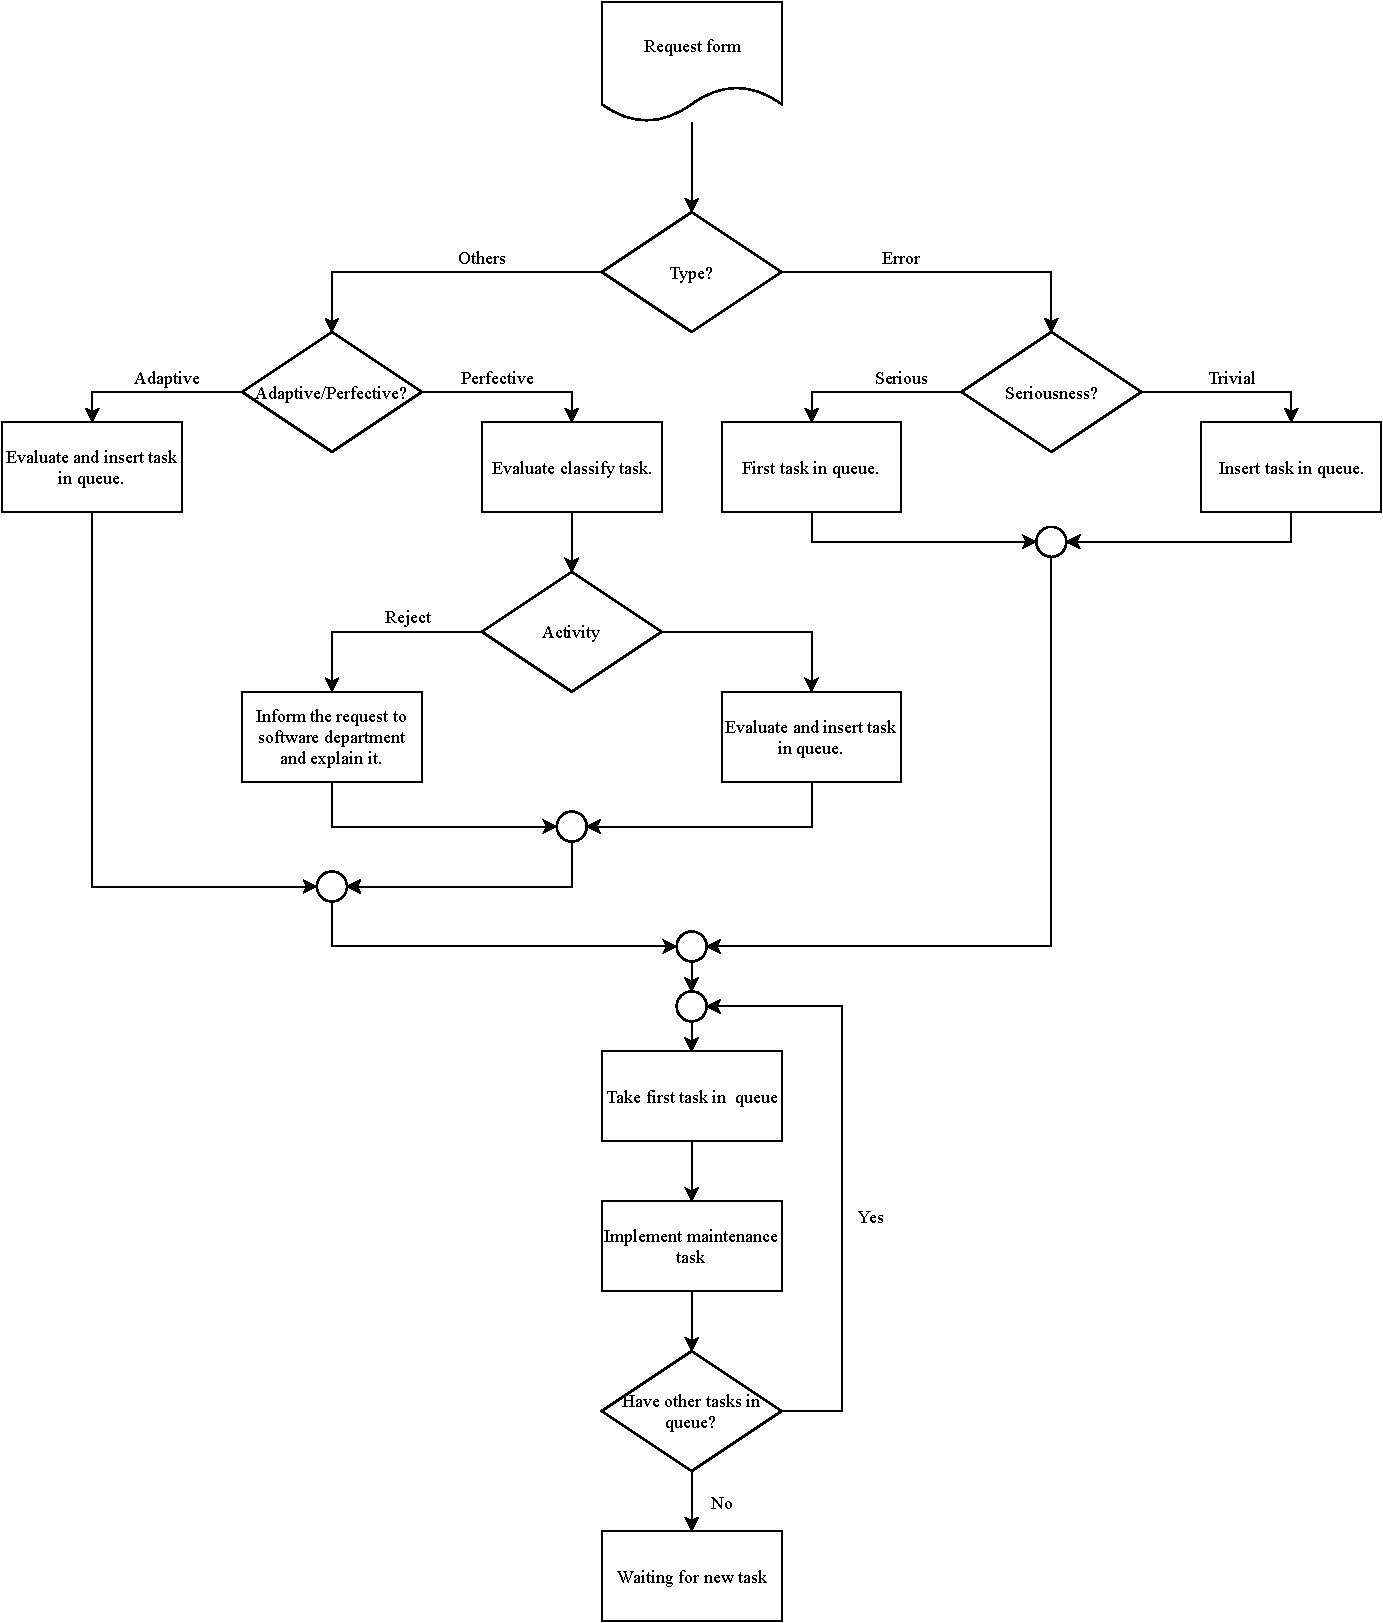
\includegraphics[width=0.9\textwidth]{Images/Chapter1/Background/Maintenance_flow/Maintenance_Flow.pdf}
	\caption[Maintenance flow model]
	{\textit{Maintenance flow model}} \label{fig:CH1_MaintenanceFlow}
\end{figure}

\clearpage

\section{Literature study}

\subsection{Event logging}
In \Cref{section:background} software maintenance can make use of event logs to improve software maintenance. It is a common practice in the software industry to record any detailed system run-time information into logs to be analysed later by developers or software engineers to solve software related problems with the system as in \Cref{tbl:CH1_EventLogsUsage} \cite{Zhu2019}.

\begin{table}[!htb]
	\centering
	\small
	\caption[Event logs usage]
	{\textit{Event logs usage}}
	\label{tbl:CH1_EventLogsUsage}
	\begin{tabularx}{\textwidth}{|l|X|}
		\hline \textbf{Usage} & \textbf{Description} \\
		\hline Debugging of software systems & Able to diagnose software failures for both testing and production environments \cite{Rong2018a}.\\
		\hline Anomaly detection & Event logs can be used to detect any abnormal system behaviour using an anomalous detection algorithm using logging data \cite{Gurumdimma2016}.  This can also be use to find any vulnerabilities in the software environment \cite{Dwyer2013}. \\
		\hline Performance diagnosis & Software performance is important to producing quality software \cite{EvangelinGeetha2007,Baccanico2014}. This is mostly performance logs of software systems which are used to monitor the software system which is useful for resource tuning, load balancing and checking system scalability \cite{Sosnowski2014} \\ 
		\hline Error and failure analysis & Event logs is used to analyse the failure behaviours of software systems which enables engineers to understand the failure modes of the system, find the root cause of these failures, prevent them and improve the reliability of the future releases of the system \cite{Cinque2013}.\\
		\hline Analysis of security alerts & In any software environment or information technology infrastructure, security is a major concern for any company \cite{Pathan2014, Dwyer2013}. It is important to know the overall security status of the software system \\
		\hline
	\end{tabularx}
\end{table}

The technique to collect numeric or textual data that describes the behaviour of a computer system is called event logging \cite{Pecchia2015, Baccanico2014}. Event logs are collected textual data containing the records of events that happened in a software system and is used for system management tasks as in \Cref{tbl:CH1_EventLogsUsage} \cite{Rong2018a, Rong2018, Baccanico2014}.

\subsection{Logging practice in software engineering}
Providing a guide for software engineers and developers to implement a suitable logging implementation in their software systems has proving to be a vital tool in both industrial use and progress of academia \cite{Rong2018a}. Guoping Rong et al.~made a study to review these logging practices published papers to improve the performance and efficiency of logging implementation. From his study he made selection criteria to include (as in \Cref{tbl:CH1_RongIncSelectionCriteria}) and exclude (as in \Cref{tbl:CH1_RongExlSelectionCriteria}) academic papers about logging practices \cite{Rong2018a,Rong2018}.\par The Rong's selection criteria obtained numerous research papers of logging practices applied in the industry by either creating a new logging mechanism or optimising existing logging mechanisms. By reviewing 41 identified papers he found that many practitioners and researchers recognises the importance of logging practice in software engineering. There is a lack of guidance to provide software engineers or developers to create or improve their own efficient logging mechanisms \cite{Rong2018a,Zhu2015}. 

\begin{table}[!htb]
	\centering
	\small
	\caption[G. Rong's inclusion selection criteria]
	{\textit{G. Rong's inclusion selection criteria \cite{Rong2018a}}}
	\label{tbl:CH1_RongIncSelectionCriteria}
	\begin{tabularx}{\textwidth}{|c|X|}
		\hline \textbf{Identification} & \textbf{Criteria} \\
		\hline I1. & Publications that investigate the methodology for logging practice. \\
		\hline I2. & Publications that investigate the tools, frameworks, systems which support logging practice. \\
		\hline I3. & Publications that propose a standard for logging practice.\\
		\hline I4. & Publications that are peer-reviewed (conference paper, journal article). \\
		\hline I5. & Publications that are primary studies on logging practice. \\
		\hline
	\end{tabularx}
\end{table}

\begin{table}[!htb]
	\centering
	\small
	\caption[G. Rong's exclusion selection criteria]
	{\textit{G. Rong's exclusion selection criteria \cite{Rong2018a}}}
	\label{tbl:CH1_RongExlSelectionCriteria}
	\begin{tabularx}{\textwidth}{|c|X|}
		\hline \textbf{Identification} & \textbf{Criteria} \\
		\hline E1. & Publications that investigate log analysis. \\
		\hline E2. & Publications that investigate the usage of logs. \\
		\hline E3. & Publications that investigate the technologies on logging user behaviors. \\
		\hline E4. & Publications that are not written in English. \\
		\hline E5. & Additionally, short papers, demo or industry publications are excluded. \\
		\hline
	\end{tabularx}
\end{table}
Software engineers and developers will need to make informed logging decisions to cover the necessary runtime information without negatively impacting the software system's performance \cite{Zhu2015,Zhu2019}. This negative impact can be attributed to by:

\begin{itemize}
	\item \textbf{Quantity of the logs:} It can become difficult to log every event in a software system as these systems will get larger and more complex during its the development life cycle \cite{Stojanov2017}. It would be bad too not log enough information during runtime as the necessary information about the event will make the postmortem analysis of the software system incomplete \cite{Zhu2015}.
	\item \textbf{Quality of the logs:}
\end{itemize}

In \Cref{fig:CH1_PushblisedPapers} shows the distribution of the 41 published papers obtained for Rong's research relating to logging practices. Event logging has an increasing important role in modern software systems, therefore the research focus on logging practices in software engineering have been increasing between 1990 and 2017.

\begin{figure}[!htb] % An h :here, t: top, b: bottom.
	\centering % cent the figure
	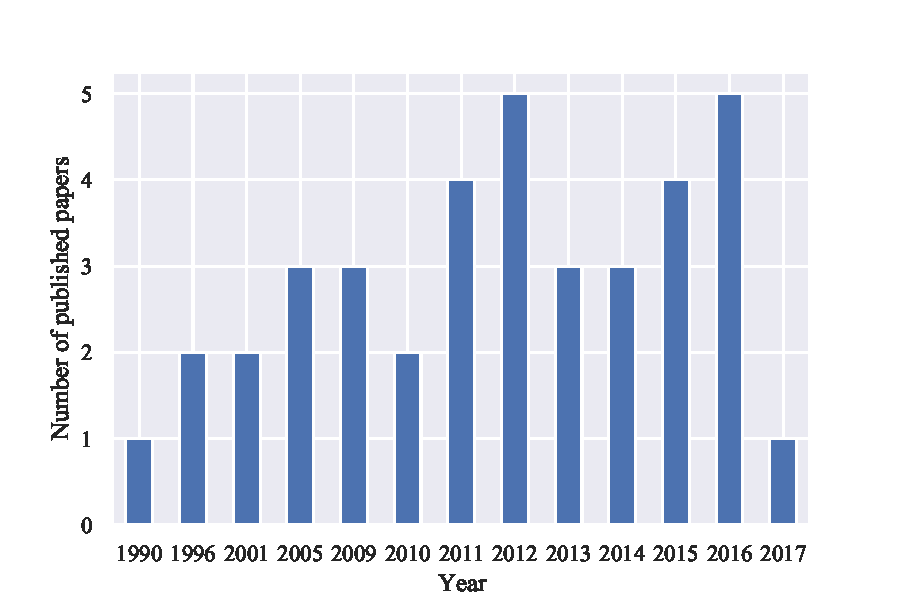
\includegraphics[width=0.9\textwidth]{Images/Chapter1/Background/Ronga2018.pdf}
	\caption[The distribution of the papers’ published years]
	{\textit{The distribution of the papers’ published years \cite{Rong2018a}}} \label{fig:CH1_PushblisedPapers}
\end{figure} 

\clearpage

\subsection{System utilisation analysis}

\clearpage

\section{Objectives of the study}
The goal of the study is to develop a logging mechanism to track user-based
activities to preform analysis of these logs to improve system maintenance in
software environment. The study is divided in two components to achieve the
primary goal which is the design and implementation of the logging mechanism
and the analysis of the system utilisation to improve system maintenance.

\subsection{Logging mechanism:}
\begin{itemize}
	\item Random text.
\end{itemize}

\subsection{Analysis of the system utilisation to improve software maintenance}
\begin{itemize}
	\item Random text.
\end{itemize}

\section{Overview of the dissertation}
\subsubsection{Chapter 1: Introduction}
This chapter contains the background of software maintenance and system
utilisation analysis.
\subsubsection{Chapter 2: Mehtodolgy}